% Chapter 1

\chapter{Introducción general} % Main chapter title

\label{Chapter1} % For referencing the chapter elsewhere, use \ref{Chapter1} 
\label{IntroGeneral}
En este capítulo se realiza una breve introducción de los elementos externos que interactúan con el sistema con la finalidad de brindar un marco de comprensión general antes de realizar un abordaje específico. También se explica el alcance y objetivos del presente trabajo.

%----------------------------------------------------------------------------------------

% Define some commands to keep the formatting separated from the content 
\newcommand{\keyword}[1]{\textbf{#1}}
\newcommand{\tabhead}[1]{\textbf{#1}}
\newcommand{\code}[1]{\texttt{#1}}
\newcommand{\file}[1]{\texttt{\bfseries#1}}
\newcommand{\option}[1]{\texttt{\itshape#1}}
\newcommand{\grados}{$^{\circ}$}

%----------------------------------------------------------------------------------------
%----------------------------------------------------------------------------------------
\section{Descargas parciales}
Según IEEE

\textit{(Guide for the Measurement of Partial Discharges in AC Electric Machinery)}
\enquote{Una DP es una descarga eléctrica que cortocircuita parcialmente el material aislante ubicado entre dos conductores. Cuando la tensión excede cierto valor crítico, se produce una ionización gaseosa transitoria en el sistema aislante, a dicha ionización se la denomina DP} \citep{IEEE:citation}

Una descarga parcial es un fenómeno de disrupción eléctrica. Se caracteriza por ser un pulso de corriente de alta frecuencia el cual se produce en el seno de un sistema aislante de una máquina o equipo eléctrico de potencia de media o alta tensión como consecuencia de la presencia de  oclusiones gaseosas, impurezas, aristas aguzadas u otras anomalıas que distorsionan la distribución de las líneas de campo eléctrico, figura \ref{fig:basicoDp}.

\begin{figure}[ht]
	\centering
	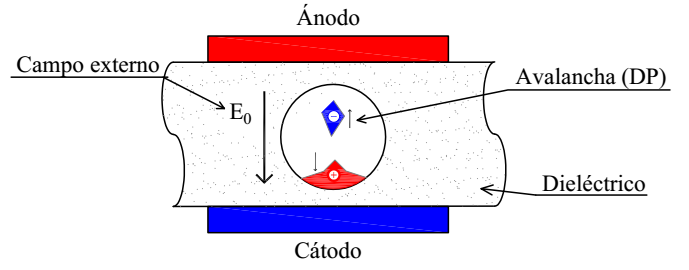
\includegraphics[width=\textwidth]{./Figures/basicoDp.png}
	\caption{Esquema básico de DP en el interior de un aislante.}
	\label{fig:basicoDp}
\end{figure}

La ocurrencia de este fenómeno provoca un deterioro del sistema aislante. Dependiendo del medio en el que este fenómeno se manifiesta y cuál sea la causa que lo origina, el deterioro del sistema puede ser acumulativo.

\section{Medidores de descargas parciales}
La técnica eléctrica más utilizada se basa en registrar las corrientes originadas por las DP en el interior del sistema aislante. La detección de estas se realiza mediante la utilización de sensores inductivos pasivos de alta frecuencia conectados en las derivaciones a tierra de los equipos que se desean ensayar.

Cuando la DP se produce en el interior del sistema aislante, las corrientes que circulan hacia tierra pasan a través del sensor inductivo; induciendo una fuerza electromotriz proporcional a la carga involucrada, figura \ref{fig:dpEjemplo}.

\begin{figure}[ht]
	\centering
	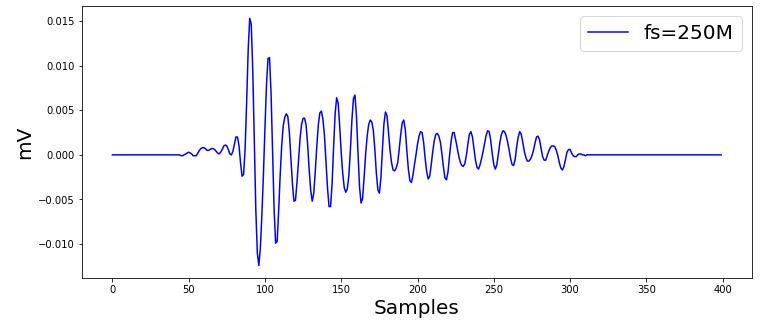
\includegraphics[width=\textwidth]{./Figures/dpEjemplo.png}
	\caption{Forma de onda de una descarga parcial capturada por un HFCT (high frequency current transformer).}
	\label{fig:dpEjemplo}
\end{figure}

Las DP registradas son representadas en un sistema de referencias en cuyo eje de ordenadas se indica la máxima amplitud del pulso y en el eje de abscisa el momento angular en que el fenómeno ocurre respecto de una senoide de referencia de 50 Hz. Por medio de la superposición de múltiples eventos sobre un mismo periodo de 50 Hz se conforma lo que se conoce en la literatura especializada como Diagrama de Magnitud - Fase o Patrón de DP, figura \ref{fig:patronEjemplo}.

\begin{figure}[!ht]
	\centering
	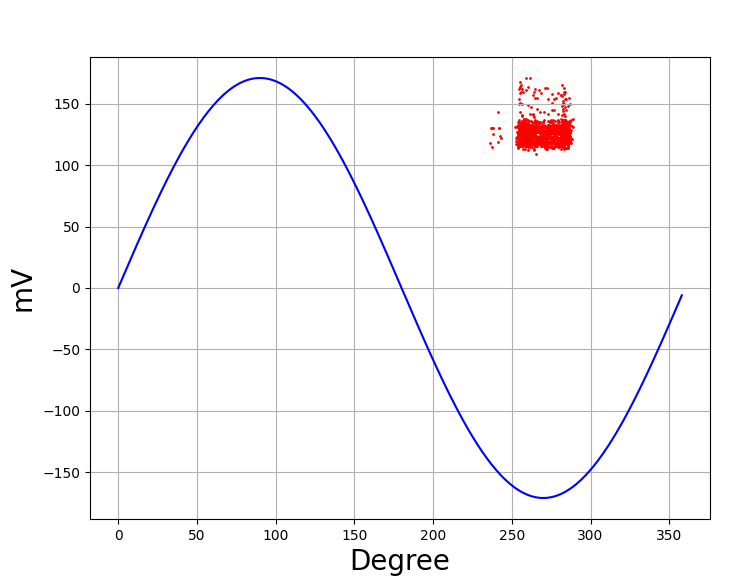
\includegraphics[width=100mm]{./Figures/patronEjemplo.png}
	\caption{Patrón de descargas parciales.}
	\label{fig:patronEjemplo}
\end{figure}

Los patrones de DP permiten identificar, por medio de su estructura, el grado de severidad de un falla \citep{Gulski:citation}. También permiten emitir un diagnóstico, ya que distintos tipos de DP tienen asociados distintos riesgos \citep{Cavallini:citation}.

Sensor inductivo

Los transformadores de corriente de alta frecuencia (HFCT), figura \ref{fig:hfct}, son sensores inductivos que dada su robustez y su sensibilidad están ampliamente difundidos como elementos captores para mediciones de DP en campo. Estos se instalan en las derivaciones a tierra de las máquinas o equipos eléctricos de potencia donde se desea medir la ocurrencia de este fenómeno.


\begin{figure}[ht]
	\centering
	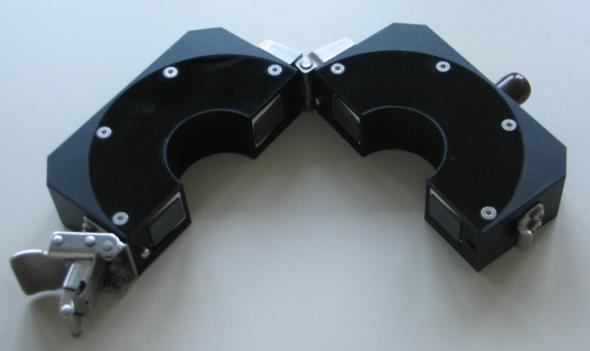
\includegraphics[width=100mm]{./Figures/hfct1.png}
	\caption{HFCT de la empresa TechImp.}
	\label{fig:hfct}
\end{figure}

\section{Estado del arte}
Actualmente existen equipos de medición de DP fabricados por empresas extranjeras como TechImp, PD Power Diagnostix u Omnicrom. Si bien esta gama de equipos abarca un amplio rango de características, ninguno proporciona una herramienta considerada de bajo costo para nuestro país, que permita a cooperativas o medianas empresas acceder a este herramienta de diagnóstico. Al mismo tiempo, este equipo proporciona una herramienta de base para implementar algoritmos propios para procesamiento \textit{over the edge}; características que no tienen los actuales equipos en el mercado. 

Equipos existentes en el mercado de características similares al equipo desarrollado:

TechImp Falcon \citep{falconWeb:1}
\begin{itemize}
\item Solución “económica” para monitoreo constante de descargas parciales.
\item Adquisición automática y generación del patrón de descargas parciales.
\item Separación de las diferentes actividades de descargas.
\item Ancho de banda 30 MHz resolución 12 bits.
\item Conexión ethernet.
\end{itemize}

\begin{figure}[h!]
	\centering
	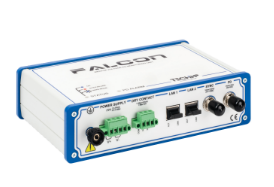
\includegraphics[width=80mm]{./Figures/arte1.png}
	\caption{Equipo Falcon de Techimp.}
	\label{fig:arte1}
\end{figure}


\vspace{15mm}
PD Power Diagnostix ICMmonitor \citep{pdWeb:1}
\begin{itemize}
\item Creación del patrón y display para visualización \textit{in-situ}.
\item Analizador de espectro.
\item Posibilidad de monitoreo remoto.
\item Conexión TCP.
\end{itemize}

\begin{figure}[h!]
	\centering
	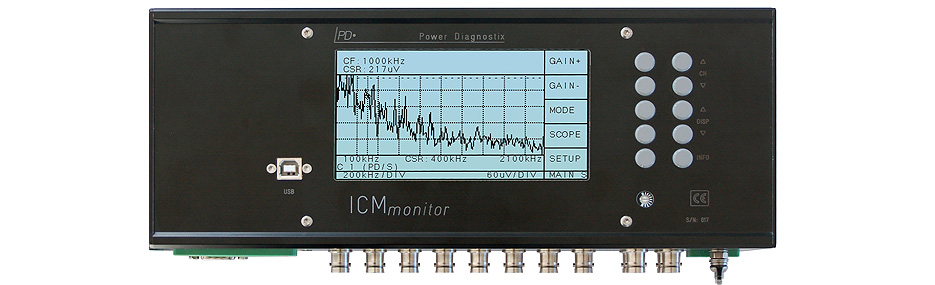
\includegraphics[width=90mm]{./Figures/arte2.png}
	\caption{Equipo ICMmonitor de Pdix.}
	\label{fig:arte2}
\end{figure}


Omicrom MPD600 \citep{mpdWeb:1}
\begin{itemize}
\item Medicion y analisis de descargas.
\item Permite grabar, analizar y mostrar las señales.
\end{itemize}

\begin{figure}[h!]
	\centering
	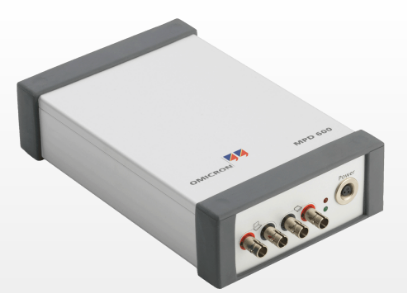
\includegraphics[width=80mm]{./Figures/arte3.png}
	\caption{MPD600 de Omnicrom.}
	\label{fig:arte3}
\end{figure}

\section{Objetivos y alcance}
\subsection{Objetivos}
El objetivo de este trabajo fue desarrollar un prototipo de un equipo adquisidor de DP de calidad, de bajo costo y de producción nacional. A su vez, se buscó crear las bases para un equipo abierto con capacidad de hacer procesamiento \textit{over the edge}. 

\subsection{Alcance}
El alcance del trabajo incluyó:
\begin{itemize}
\item El desarrollo del prototipo del producto.
\item El desarrollo del firmware.
\item El diseño del circuito esquemático.
\item Confección de un manual de uso.
\item Pruebas de validación y verificación.
\end{itemize}

